\section{Other Requirements}

\subsection{Appendix A: Glossary}

This glossary provides definitions for the technical and medical terminology used throughout this SRS document to ensure a consistent understanding among all stakeholders.

\keepXColumns 
\begin{tabularx}{\textwidth}{l L}
	\caption{Glossary of Terms and Abbreviations} \label{tab:glossary} \\
	
	\toprule
	\textbf{Term} & \textbf{Definition} \\
	\midrule
	\endfirsthead
	
	\multicolumn{2}{c}{{\bfseries \tablename\ \thetable{} -- Continued from previous page}} \\
	\toprule
	\textbf{Term} & \textbf{Definition} \\
	\midrule
	\endhead
	
	\bottomrule
	\endfoot
	
	\textbf{SRS} & Software Requirements Specification: A formal document that describes the functional and non-functional requirements of the system. \\ \addlinespace
	\textbf{MVC} & Model-View-Controller: A software architectural pattern that separates the application into Data (Model), Logic (Controller), and Interface (View). \\ \addlinespace
	\textbf{SPA} & Single Page Application: A web application that dynamically updates the current page rather than loading new pages from a server (e.g., using Vue.js). \\ \addlinespace
	\textbf{RBAC} & Role-Based Access Control: A security mechanism that restricts system access based on user roles (Admin, Doctor, Receptionist). \\ \addlinespace
	\textbf{EMR} & Electronic Medical Record: A digital version of a patient’s medical history, including diagnoses and prescriptions. \\ \addlinespace
	\textbf{PDO} & PHP Data Objects: A consistent way to access databases in PHP with protection against SQL injection. \\ \addlinespace
	\textbf{Audit Trail} & (Active Log) A chronological record of system activities affecting operations or events. \\ \addlinespace
	\textbf{Scalability} & The capability of the system to handle growth in users, data, or workload. \\ \addlinespace
	\textbf{Business Rules} & The logic and constraints governing clinic operations (e.g., preventing schedule overlaps). \\ \addlinespace
	\textbf{JSON} & JavaScript Object Notation: A lightweight format for data exchange between PHP backend and Vue.js frontend. \\ \addlinespace
	\textbf{UI/UX} & User Interface / User Experience: The visual and interactive experience of the system. \\
	
	\bottomrule
\end{tabularx}
\newpage
\subsection{Appendix B: Analysis Models}

\subsubsection{Use Case Diagrams}
\paragraph{7.2.1.1 High-level:}
The high-level use case diagram provides an abstract representation of the CMS, identifying primary actors and the central authentication mechanism.
\begin{figure}[H]
	\centering
	\includegraphics[width=\textwidth]{diagrams/UC_overview.pdf}
	\caption{High-Level Use Case Diagram}
\end{figure}

\paragraph{Actors}

\begin{itemize}
	\item \textbf{Admin} — Responsible for system configuration
	\item \textbf{Receptionist} — Appointment coordinator
	\item \textbf{Patient} — Service beneficiary
	\item \textbf{Doctor} — Healthcare service provider
\end{itemize}

\begin{table}[H]
	\centering
	\renewcommand{\arraystretch}{1.4} 
	\begin{tabularx}{\textwidth}{l L}
		\toprule
		\textbf{Use Case} & \textbf{Functional Description} \\ 
		\midrule
		Login & Secure authentication gate required for all internal operations. \\ \addlinespace
		Manage System & Configuration of clinic parameters and security logs. \\ \addlinespace
		Manage Appointments & The lifecycle of booking, scheduling, and confirmation. \\ \addlinespace
		Manage Medical Records & Centralized management of patient clinical data. \\ 
		\bottomrule
	\end{tabularx}
\end{table}

%===================
% 7.2.1.2	Admin 
%===================
\newpage
\paragraph{7.2.1.2 The Admin Role:}
	The Admin maintains full authority over the system's structural data, including staff accounts and service pricing.

\begin{figure}[H]
	\centering
	\includegraphics[width=0.85\textwidth]{diagrams/UC_admin.pdf}
	\caption{Admin Use Case Diagram}
\end{figure}

\begin{table}[H]
	\centering
	\renewcommand{\arraystretch}{1.3}
	\begin{tabularx}{\textwidth}{l X l}
			\caption{Admin Use Case } \label{tab:glossary} \\
		\toprule
		\textbf{Use Case} & \textbf{Description} & \textbf{Included Actions} \\
		\midrule
		Manage Users & Staff account lifecycle management & Add/Update/Deactivate \\
		Manage Doctors & Specialized professional data control & Medical Credentials \\
		Manage Specialties & Defining clinic medical departments & Add/Update \\
		Manage Services & Controlling services and pricing lists & Set Pricing \\
		View Reports & Extracting analytical and financial data & Activity Logs \\
		\bottomrule
	\end{tabularx}
\end{table}
%===================
% 	Doctor 
%===================
\newpage
\paragraph{7.2.1.3 The Doctor Role:}
	Focused on clinical efficiency, this module enables doctors to document consultations and manage medical history.

\begin{figure}[H]
	\centering
	\includegraphics[width=0.85\textwidth]{diagrams/UC_doctor.pdf}
	\caption{Doctor Use Case Diagram}
\end{figure}

\begin{table}[H]
	\caption{Doctor Use Case } 
	\centering
	\renewcommand{\arraystretch}{1.3}
	\begin{tabularx}{\textwidth}{l X l}
		\toprule
		\textbf{Use Case} & \textbf{Description} & \textbf{Technical Note} \\
		\midrule
		View Daily List & Access list of scheduled patients & Schedule-link \\
		Set Availability & Manage working hours and leaves & Real-time update \\
		Patient History & Review previous clinical notes & Read access \\
		Add Diagnosis & Document current medical condition & Write access \\
		Create Prescription & Generate digital medication orders & Integrated flow \\
		Reset Password & Self-service credential recovery & Extend relationship \\
		\bottomrule
	\end{tabularx}
\end{table}
%===================
% Patient 
%===================
\newpage
\paragraph{7.2.1.4 The Patient Role:}
	The Patient module empowers end-users to manage their healthcare journey autonomously.

\begin{figure}[H]
	\centering
	\includegraphics[width=0.85\textwidth]{diagrams/UC_patient.pdf}
	\caption{Patient Use Case Diagram}
\end{figure}


\begin{table}[H]
	\caption{Patient Use Case } 
	\centering
	\renewcommand{\arraystretch}{1.3}
	\begin{tabularx}{\textwidth}{l X l}
		\toprule
		\textbf{Use Cases} & \textbf{Description} & \textbf{Category} \\
		\midrule
		Register/Login & Secure account management & Access Control \\
	Book/Cancel/View & Full control over personal bookings & Appointments \\
		View Records/Labs & Secure access to medical documentation & Health Records \\
		Invoices/Pay & Managing dues and online payments & 	Financials \\
		\bottomrule
	\end{tabularx}
\end{table}

%===================
% Receptionist 
%===================
\newpage
\paragraph{7.2.1.5 The Receptionist Role:}
This role manages the "Front-Desk" operations, acting as the primary coordinator for clinic traffic.

\begin{figure}[H]
	\centering
	\includegraphics[width=0.85\textwidth]{diagrams/UC_receptionist.pdf}
	\caption{Receptionist Use Case Diagram}
\end{figure}


\begin{table}[H]
	\caption{Receptionist Use Case } 
	\centering
	\renewcommand{\arraystretch}{1.3}
	\begin{tabularx}{\textwidth}{l X l}
		\toprule
		\textbf{Cases} & \textbf{Description} & \textbf{Category} \\
		\midrule
		Search/Register  & Registering and verifying patient identity & Patient Intake \\
		Create/Reschedule & Managing the doctor's calendar & Scheduling \\
		Invoice/Receipt & Converting visits to financial claims & 	Billing \\
		Physical arriva & Updating arrival status (Check-In) & 	Operational Checkl \\
		\bottomrule
	\end{tabularx}
\end{table}
%=========================
% 	Activity Diagram
%=========================
\newpage
\subsubsection{Activity Diagram}

\paragraph{7.2.2.1 Admin Activity Diagram}
This Activity Diagram illustrates the high-level operational flow for the System Administrator. 
It utilizes swimlanes to categorize actions between the Admin, the System logic, and the Database, 
providing a clear view of how administrative tasks are processed.

\begin{figure}[H]
	\centering
	\includegraphics[width=\textwidth]{diagrams/ACT-admin.pdf}
	\caption{Admin Activity Diagram — Clinic Management System}
\end{figure}

\paragraph{Workflow Explanation}
	\begin{enumerate}
	\item \textbf{Dashboard Initialization}  
	Each session starts with automatic statistical data loading, providing immediate insights such as revenue and patient count.
	
	\item \textbf{Decision Branching}  
	The workflow splits into three major administrative domains:
	
	\begin{itemize}
		\item \textbf{Identity \& Access Management:} Managing doctors and staff lifecycle (Add, Edit, Deactivate).
		\item \textbf{Business Intelligence:} Generating and exporting reports based on time filters.
		\item \textbf{Global Configuration:} Defining clinic operational settings such as working hours and metadata.
	\end{itemize}
	\item \textbf{Consolidated Persistence}Regardless of the chosen path, all workflows converge at the Database lane for a synchronized "Save and Log" operation, ensuring that the Audit Trail is never bypassed.
\end{enumerate}

%=========================
% 	Patient Appointment Booking (Guest Flow) Activity Diagram
%=========================


\paragraph{7.2.2.2 Patient Appointment Booking (Guest Flow) Activity Diagram}
This Activity Diagram maps the autonomous booking journey for guest patients. It emphasizes system resilience and automated guidance through conditional logic and feedback loops.

\begin{figure}[H]
	\centering
	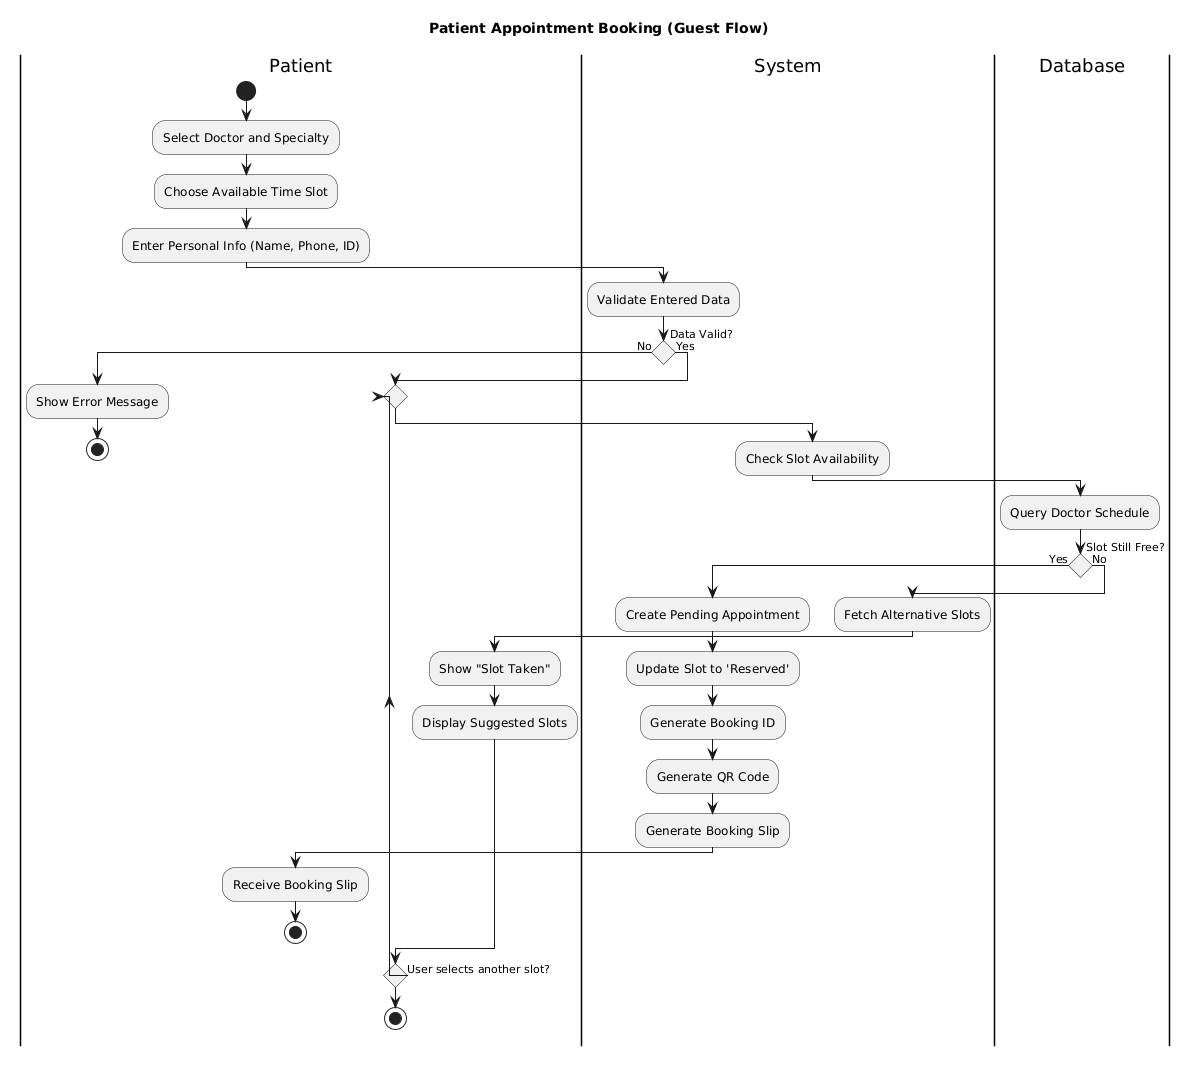
\includegraphics[width=\textwidth]{diagrams/ACT-book-appointment.png}
	\caption{Patient Appointment Booking (Guest Flow) Activity Diagram — Clinic Management System}
\end{figure}

	\begin{enumerate}
		\item \textbf{Proactive Validation} The system performs immediate data validation and secondary availability checks in the Database lane. This ensures that the record is only created if the time slot remains vacant at the exact moment of submission.
		\item \textbf{Technological Integration} The workflow features an automated QR Code generation process. By encoding a unique Booking ID, the system provides the patient with a digital credential that bridges the gap between the online portal and the physical clinic check-in. 
		\item \textbf{Intelligent Recovery (The "Slot Taken" Loop} In the event of a concurrency conflict (where a slot is taken mid-process), the system does not simply terminate. Instead, it fetches Suggested Other Slots, allowing the user to re-route their request without restarting the entire form. 
		\item \textbf{End-to-End Automation} The process concludes with a downloadable Booking Slip, ensuring the patient has tangible proof of their reservation.
	\end{enumerate}






%=========================
% 	Medical Examination And Consultation Flow Activity Diagram
%=========================
\newpage

\paragraph{7.2.2.3 Medical Examination And Consultation Flow Activity Diagram}
	This Activity Diagram illustrates the clinical workflow during a patient consultation. It highlights the transformation of physical observations into structured digital medical records through a collaborative process between the Doctor, the System, and the Database.
\begin{figure}[H]
	\centering
	\includegraphics[width=\textwidth]{diagrams/ACT-medical-examination.pdf}
	\caption{Medical Examination And Consultation Flow Activity Diagram}
\end{figure}

\paragraph{Workflow Explanation}
\begin{enumerate}
	\item \textbf{Information Retrieval}  
	The process is data-driven; the System automatically retrieves the patient’s historical records the moment a selection is made, ensuring the Doctor has a complete longitudinal view of the patient’s health before the examination begins.
	\item \textbf{Decision-Based Prescription}  
	The workflow incorporates a conditional branch for medication. If a prescription is required, the system provides a specialized interface for entry; otherwise, it proceeds directly to data validation.	
	\item \textbf{Integrity and Persistence}  
	All clinical findings (Diagnosis and Treatment) undergo a system validation check before being committed to the DBMS. This ensures that the medical record is updated accurately and remains available for future consultations.
	\item \textbf{Professional Closure}
	The activity concludes with the generation of a Digital Prescription and a final confirmation by the Doctor, reinforcing the professional responsibility and communication with the patient.
\end{enumerate}
%=========================
% 	 Patient Billing and Payment
%=========================

\newpage
\paragraph{7.2.2.4Patient Billing and Payment Activity Diagram}
	This Activity Diagram maps the financial settlement process at the end of a medical visit. It highlights the system's ability to handle dynamic pricing based on insurance coverage and ensures synchronous updates across the financial and clinical modules..
\begin{figure}[H]
	\centering
	\includegraphics[width=\textwidth]{diagrams/ACT-patient-billing-payment.pdf}
	\caption{Patient Billing and Payment Activity Diagram}
\end{figure}

\paragraph{Workflow Explanation}
\begin{enumerate}
	\item \textbf{Dynamic Billing Logic}
	The workflow starts with an automated fetch of all services rendered during the visit. The system integrates a conditional logic for Insurance Coverage, allowing for real-time discount applications before the final invoice is generated.
	\item \textbf{Error Handling and Resilience}
	The diagram incorporates a failure branch for payment processing. If a transaction is declined, the system guides the Receptionist to inform the patient and retry, preventing "orphan" invoices that are neither paid nor cancelled.
	\item \textbf{Database Synchronization}
	Upon successful payment, the Database lane performs a dual update: recording the financial transaction for accounting and marking clinical services as "Billed" to prevent duplicate charging.
	\item \textbf{Document Lifecycle}
	The process concludes with the generation and printing of both the Invoice and the Receipt, providing a complete audit trail for both the patient and the clinic administration.
\end{enumerate}
% ==========================================
% Receptionist Activity Diagram
% ==========================================
\newpage
\paragraph{7.2.2.5 Receptionist Activity Diagram}
This Activity Diagram details the initial reception phase, focusing on the transition from "Appointment Booking" to "Physical Presence." It highlights the system's multi-channel search capabilities and data reconciliation logic.
\begin{figure}[H]
	\centering
	\includegraphics[width=\textwidth]{diagrams/ACT-receptionist.pdf}
	\caption{Receptionist Activity Diagram}
\end{figure}

\paragraph{Workflow Explanation}
	\begin{enumerate}
	\item \textbf{Multi-Identifier Search}
	The workflow showcases a robust search logic within the System lane. By allowing identification via Phone, Name, ID, or QR Code, the system minimizes wait times and human error during the peak check-in hours.
	\item \textbf{Status Synchronization}
	When an appointment is found, the system performs an automated status update to "Arrived." This informs the Doctor’s dashboard in real-time that the patient is ready in the waiting area.
	\item \textbf{Profile Reconciliation}The diagram intelligently handles three entry scenarios:
	\begin{itemize}
		\item Pre-booked patients with existing profiles.
		\item Returning patients without a current appointment.
		\item New "Walk-in" patients requiring a full profile creation.
	\end{itemize}
	\item \textbf{Final Documentation}
	The process culminates in the Database lane for record persistence, followed by the generation of a Visit Slip, ensuring the patient has a physical or digital reference for their turn.
\end{enumerate}
